\documentclass[11pt]{article}

\usepackage{amsmath}
\usepackage{amssymb}
\usepackage{float}
\usepackage{geometry}
\usepackage{tikz}
\usetikzlibrary{patterns,decorations.pathreplacing}
\usetikzlibrary{shapes.geometric, arrows.meta, positioning,
decorations.pathmorphing}
\usepackage{graphicx}
\usepackage{hyperref}

\geometry{margin=1in}
\setlength{\parindent}{0pt}

\title{Measuring Planck’s Constant using the Photoelectric Effect}
\author{Spandan Suthar and Malachi Williams, with additional data
provided by Timo Peschken}
\date{September 30, 2025}

\begin{document}

\maketitle

\section{Goal}

We produce an experiment that investigates the relationship between
photons' wave frequencies and their energies. We configure a system
that liberates electrons from the surface of a metal using the
photoelectric effect, using lights of several frequencies. By
measuring the sensitivity of these electrons' kinetic energies to the
frequency of light used to induce their escape from the metal, we
determine the factor a photon's frequency must be scaled by to obtain
its energy, known as Planck's constant $h$. As a byproduct of our
procedure, we identify the effective work function of the metal
the electrons were freed from. We also investigate the relationship between
a photocurrent produced and the retarding voltage applied to the
photocurrent-carrying electrons.

\section{Introduction and Background}

The photoelectric effect is a phenomenon during which photons come into
contact with the surface of a material and free electrons from the
material's potential well [2]. Electrons occupy bound states in the
in a metal material with a variety of energy levels---in other words, states at
varying depths in the potential well. The maximum energy level is labeled the
Fermi energy $\epsilon$ [2]. We define the work function of a metal $W$
as the energy required to free an electron at the Fermi energy from
its bound state, making it a conduction electron. In other words, the work
function of a metal is the positive difference between the level of
zero potential energy and the Fermi energy [2].

% TODO: can we say the electrons are at differing levels because of Pauli E?

\vspace{1em}

\begin{figure}[H]
  \begin{center}
    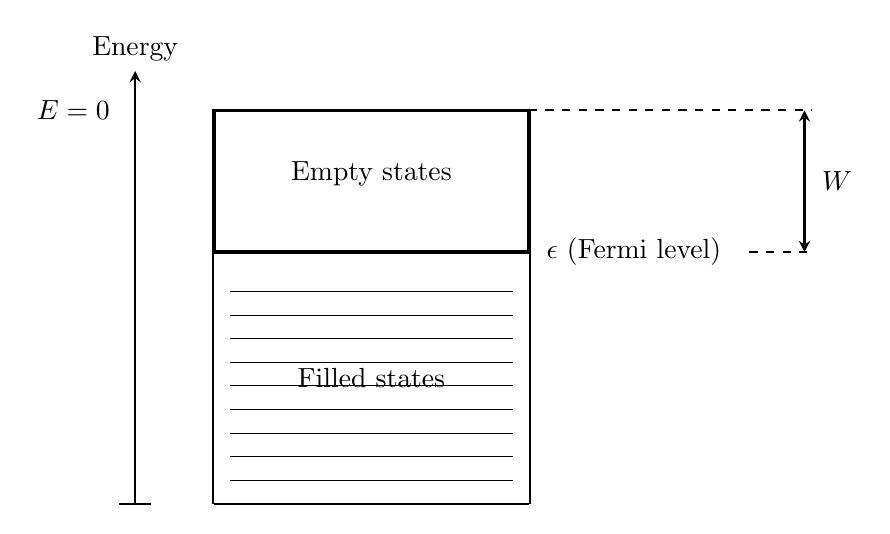
\begin{tikzpicture}[>=stealth]

      % Potential well boundaries
      \draw[very thick] (0,0) -- (0,5) -- (4,5) -- (4,0);

      % Fill the Fermi sea
      \fill[white] (0,0) rectangle (4,3.2);

      % Draw energy levels in the filled region
      \foreach \y in {0.3,0.6,...,3.0}
      \draw[thin] (0.2,\y) -- (3.8,\y);

      % Fermi level
      \draw[very thick] (0,3.2) -- (4,3.2);
      \draw[dashed, thick] (6.8,3.2) -- (7.6,3.2);
      \node[right] at (4.1,3.2) {$\epsilon$ (Fermi level)};

      % Vacuum level
      \draw[dashed, thick] (4,5) -- (7.6,5);
      \node[left] at (-1.2,5) {$E = 0$};

      % Work function arrow
      \draw[<->, thick] (7.5,3.2) -- (7.5,5);
      \node[right] at (7.6,4.1) {$W$};

      % Energy axis
      \draw[->, thick] (-1,0) -- (-1,5.5);
      \node[above] at (-1,5.5) {Energy};

      % Zero energy level
      \draw[thick] (-1.2,0) -- (-0.8,0);

      % Filled states label
      \node at (2,1.6) {Filled states};

      % Empty states label
      \node at (2,4.2) {Empty states};

      \draw[thick] (0,0) -- (4,0);

    \end{tikzpicture}
    \caption{Energy levels in a metal, showing the Fermi
    level, work function, and filled and empty states.}
    \label{fig:energy_levels}
  \end{center}
\end{figure}

\vspace{1em}

When a photon frees a bound electron in such a manner, the electron
inherits the photon's energy $E$, equal to the photon's
frequency $f$ up to a factor of $h$ [2]:
\begin{equation}
  \label{eq:photon_energy}
  E = hf
\end{equation}

The frequency of a photon $f$ is related to its wavelength $\lambda$
and the speed of light in a vacuum $c$ by [1, 2]:
\begin{equation}
  \label{eq:wave_equation}
  c = \lambda f
\end{equation}

An electric potential difference between an anode and a cathode creates a
potential gradient from high potential $V_c$ to low potential $V_a$,
producing a negative voltage jump $V_a - V_c$ from the cathode to the
anode [2].

\vspace{1em}

The potential energy of a particle of charge $q$ at a
point in space where the electric potential is $V_0$ is [2]:

\begin{equation}
  \label{eq:potential_energy}
  U_0 = q V_0
\end{equation}

\vspace{1em}

The relationship between the potential energy a photoelectron
originally at the Fermi level must accrue to be stopped by a
potential difference $\Delta V$, the wavelength $\lambda$ of the
photon, the work function $W$ of the metal, the speed of light $c$,
the fundamental charge $e$, and
and Planck's constant $h$ is:
\begin{equation}
  \label{eq:photoelectric}
  -e \Delta V = eV_s = \frac{hc}{\lambda} - W
\end{equation}

where we introduce a positive quantity $V_s$, the stopping voltage,
such that $V_s = -\Delta V$ [2].

\section{Procedure}

We establish a cathode-anode pair with the cathode's potential $V_c$
held at the ground potential and the anode's potential $V_a$ at a
potential we can adjust
using a power supply. Applying \eqref{eq:potential_energy}, electrons
forced to pass
from the cathode to the
anode against the potential gradient accrue additional positive potential
energy $q\Delta V = -e(V_a - V_c)$ upon reaching the anode, where $e$ is the
fundamental charge. By conservation of energy principles, the electron's
kinetic energy has decreased by $q\Delta V$ during this process.
Thus, as we increase $V_c$, the current measured through the
picoammeter decreases as photoelectrons of lower kinetic energies are
no longer able to reach the anode; these electrons' kinetic energies are less
than or equal to $q\Delta V$.

\vspace{1em}

Before running our experiment to determine Planck's constant, we
investigate the relationship between the anode-cathode retarding
voltage and the photoelectric current remaining after the
photoelectrons cross the voltage jump. We measure the current
produced by 570nm light at varying voltages of the anode.

\vspace{1em}

At the point where the current is 0nA, the electrons of the
highest kinetic energies are just able to reach the anode. These
electrons, having the highest kinetic energies of those in the
photocurrent produced, correspond to electrons originally at the Fermi level
and requiring the smallest contribution from the photon-supplied
energy to escape the well.

\vspace{1em}

We obtain 9 LED lights of different wavelengths. A spectrometer
provides an empirical intensity vs. wavelength curve for each light,
to which we fit Gaussian models. The Gaussian models' $1\sigma$
regions provide the
full width at half maximum boundaries of the light's wavelength
distribution, while the maximum-intensity wavelength from the points
provided by the spectrometer provides the light's wavelength.
For the wavelengths of light in our
sample set, we configure an initial photocurrent of $(5.21 \pm 0.02)$
nA at zero voltage by adjusting the light's intensity. We then
increase the voltage gap between the anode and cathode until we
achieve the zero-current configuration. We record the stopping
voltage $V_s$ corresponding to this zero-current configuration.

\vspace{1em}

This
allows us to plot empirical
samples of the relationship between $-e\Delta V$ and
$\frac{c}{\lambda}$ from \eqref{eq:photoelectric}.
The slope of a linear regression
model fit to this dataset produces $h$, our experimental value for
Planck's constant. We do not calculate $W$, attributing an
extrapolated intercept
appearing during linear regression to $W$.

\vspace{1em}

\begin{figure}[H]
  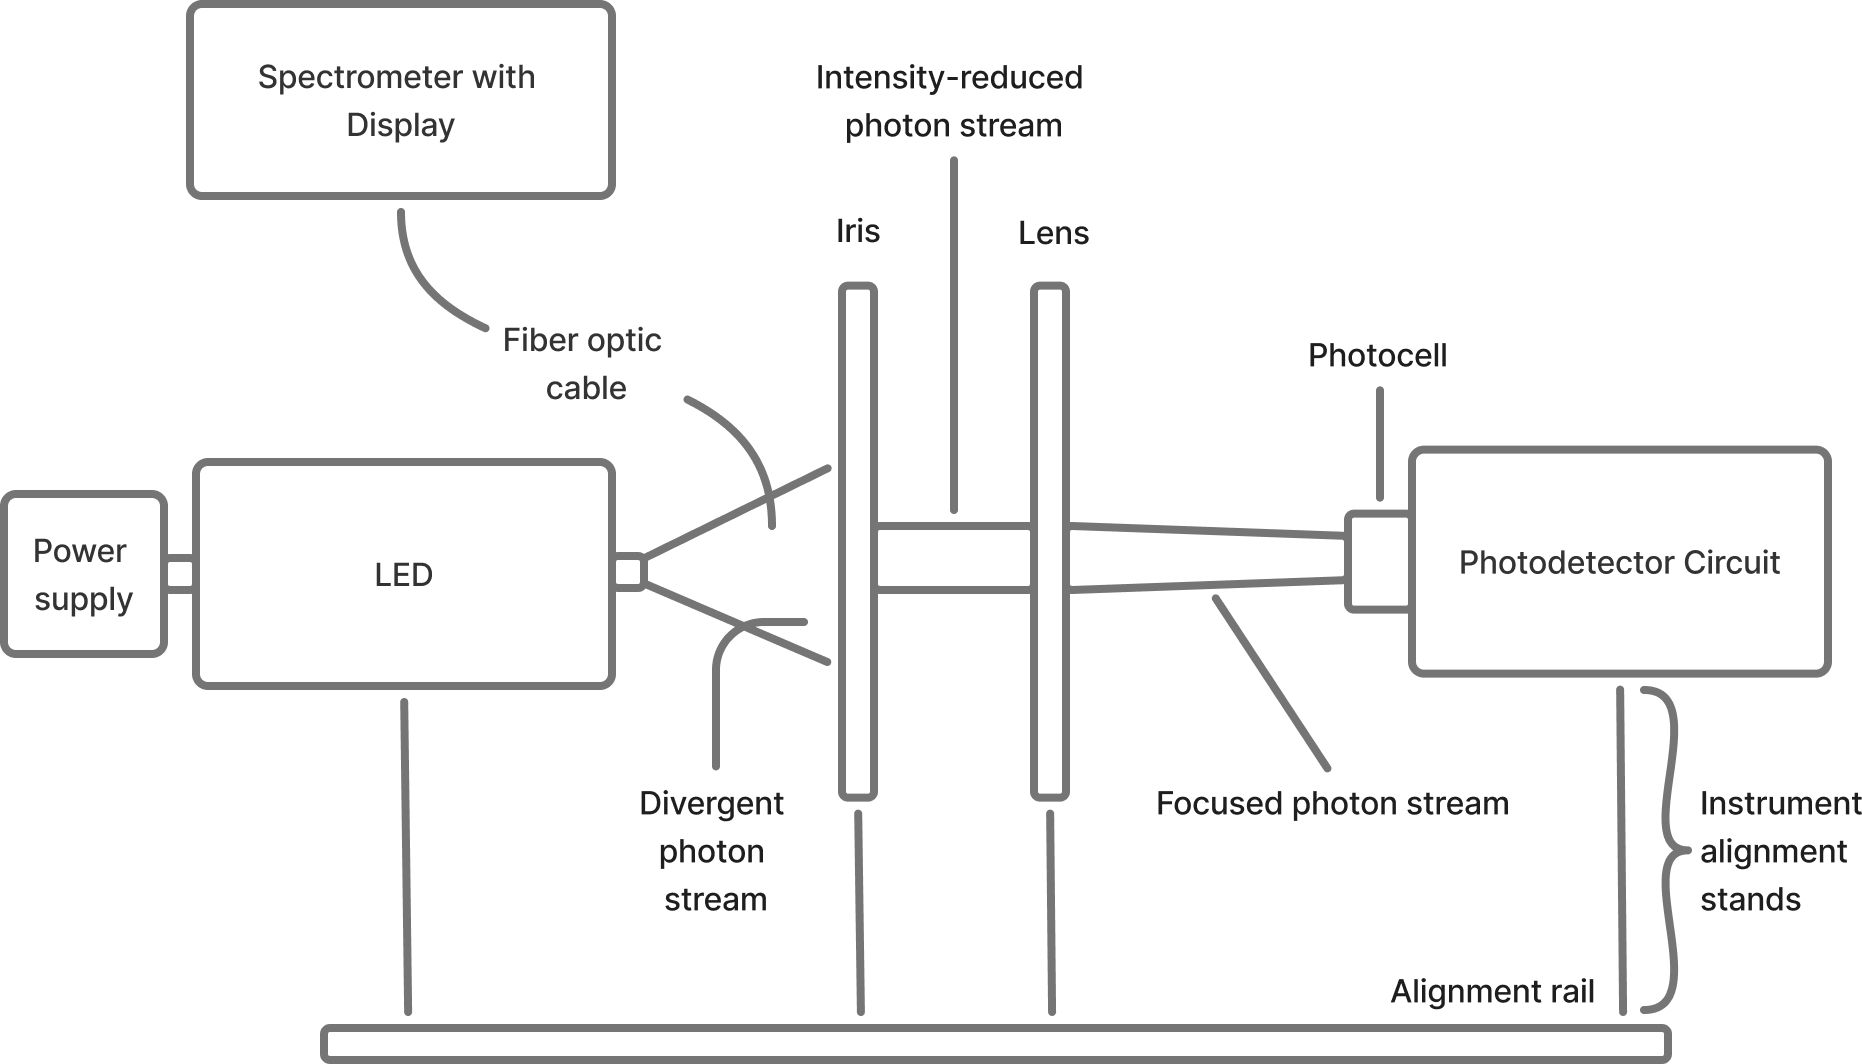
\includegraphics[width=0.75\textwidth]{../rail.png}
  \centering
  \caption{Optical rail system for inducing a photocurrent using
    LEDs. An LED faces an iris, used to control light intensity. We use a
    lens to focus the light onto a photocell linked to a
    photodetector circuit. Instruments
    are mounted on stands constrained to a rail to allow for
    alignment adjustments.
    A spectrometer
    with a fiber optic cable is used to measure intensity vs.
    wavelength relationships
  for light emitted by each LED.}
  \label{fig:spectrometer_system}
\end{figure}

\begin{figure}[H]
  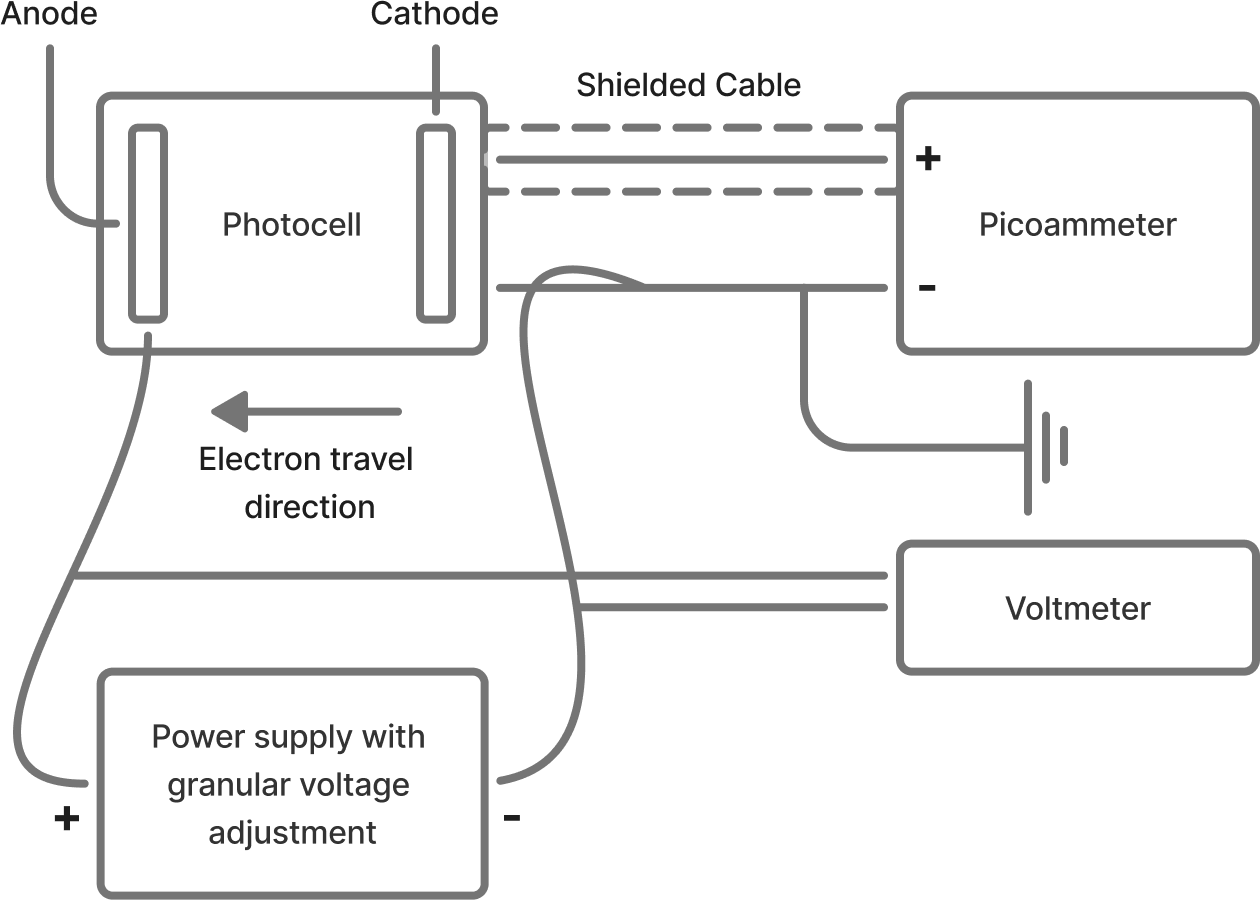
\includegraphics[width=0.57\textwidth]{../circuit.png}
  \centering
  \caption{Expanded view of the photodetector circuit. Electrons are
    liberated from the photocell and flow from the grounded cathode
    to the voltage-controlled anode. The
    resulting photocurrent is measured by a picoammeter and a voltmeter
  provides monitoring of the voltage across the diode [2].}
  \label{fig:circuit}
\end{figure}

\section{Results and Analysis}

The voltages and corresponding currents resulting from our
preliminary voltage-current experiment are shown in Table
\ref{tab:voltage_current} and plotted in Figure \ref{fig:voltage_current_plot}.

\begin{table}[H]
  \centering
  \begin{tabular}{cc}
    \hline
    Voltage (V), all $\pm$ 0.04 V & Current (nA), all $\pm$ 0.02 nA \\
    \hline
    $-3.09$ & $68.5$ \\
    $-2.75$ & $66.94$ \\
    $-2.56$ & $65.57$ \\
    $-2.25$ & $64.01$ \\
    $-2.00$ & $62.4$ \\
    $-1.75$ & $60.65$ \\
    $-1.50$ & $58.61$ \\
    $-1.25$ & $55.93$ \\
    $-1.00$ & $51.91$ \\
    $-0.75$ & $46.33$ \\
    $-0.50$ & $38.14$ \\
    $-0.25$ & $28.48$ \\
    $0.00$ & $16.14$ \\
    $0.25$ & $6.23$ \\
    $0.30$ & $3.03$ \\
    $0.40$ & $0.99$ \\
    $0.50$ & $0.26$ \\
    $0.60$ & $0.03$ \\
    $0.70$ & $-0.02$ \\
    $1.00$ & $-0.04$ \\
    $2.00$ & $-0.05$ \\
    $3.00$ & $-0.05$ \\
    \hline
  \end{tabular}
  \caption{The voltages applied to the photoelectrons and the
  corresponding currents after the photoelectrons cross the voltage jump.}
  \label{tab:voltage_current}
\end{table}

\begin{figure}[H]
  \centering
  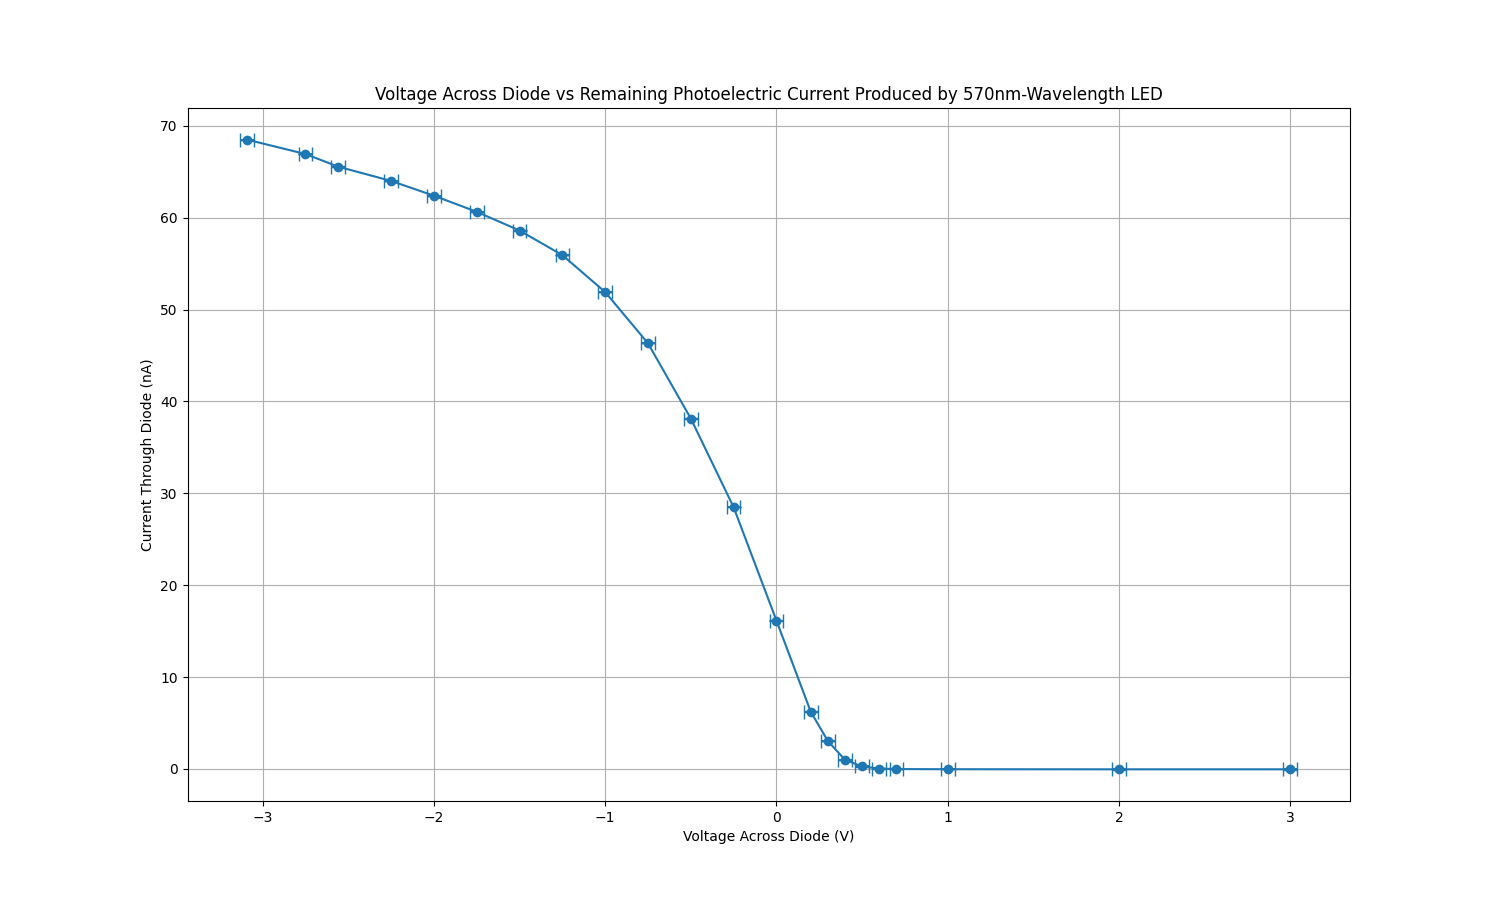
\includegraphics[width=0.8\textwidth]{../../homework1/voltage_current_plot.png}
  \caption{A plot of our measured values of the anode-cathode voltage and the
    corresponding currents after the photoelectrons cross the voltage
  jump, from Table \ref{tab:voltage_current}.}
  \label{fig:voltage_current_plot}
\end{figure}

\begin{figure}[H]
  \centering
  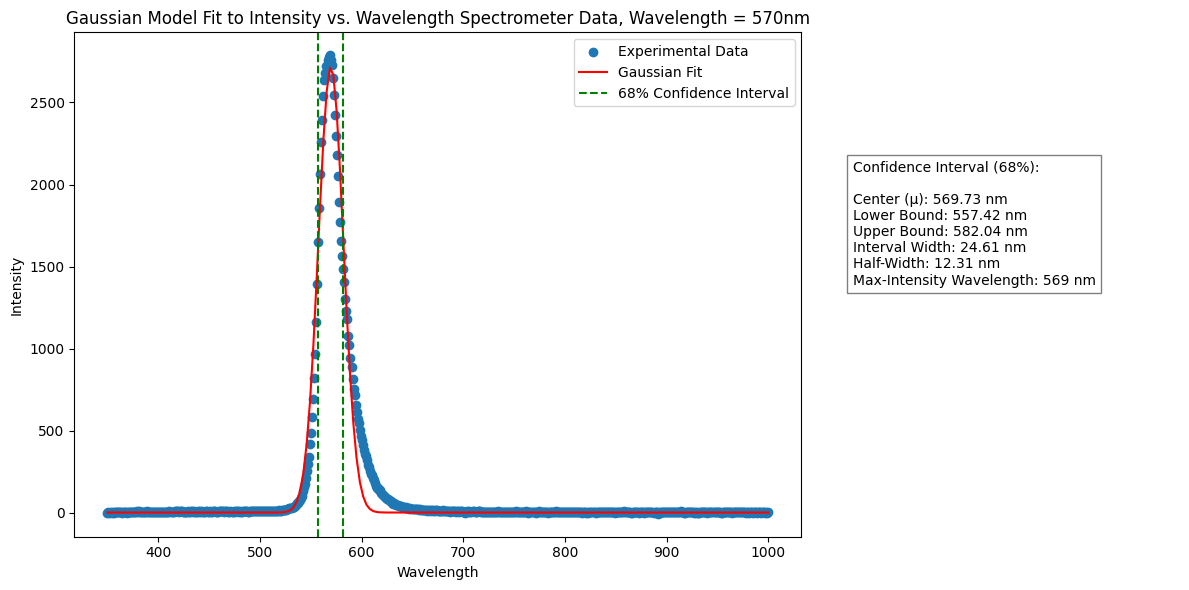
\includegraphics[width=0.8\textwidth]{../gaussian.png}
  \caption{An example of a Gaussian model fit to intensity vs.
    wavelength spectrogram data. Note that the 68\% confidence interval provides
  double the uncertainty of the maximum-intensity wavelength.}
  \label{fig:voltage_current_plot}
\end{figure}

Our measured values of the light wavelengths and the corresponding
stopping voltages are shown in Table \ref{tab:photoelectric}. We plot
our measured values of $-e\Delta V$ versus $\frac{c}{\lambda}$
in Figure \ref{fig:photoelectric_plot} and fit a linear trend line to
the data. We also perform a pointwise analysis of the dataset in table
\ref{tab:photoelectric}, using \eqref{eq:photoelectric} to compute
$h = \frac{\lambda}{c}(W + eV_s)$ for each light using the empirical value for
$W$ from the linear regression fit.
These results are also shown in Table \ref{tab:photoelectric} and
plotted in Figure \ref{fig:pointwise_h_values}.

\begin{table}[h]
  \centering
  \begin{tabular}{ccccc}
    \hline
    Max Wavelength (nm) & Stopping & $h$\\
    & Voltage ($V_s$) & ($\times 10^{-34}$ J·s) \\
    \hline
    $438.0 \pm 3.0$ & $1.2635 \pm 0.0001$ & $6.57 \pm 0.18$ \\
    $466.0 \pm 13.0$ & $1.1400 \pm 0.0001$ & $6.68 \pm 0.26$ \\
    $506.0 \pm 12.0$ & $0.8612 \pm 0.0001$ & $6.50 \pm 0.25$ \\
    $519.0 \pm 14.0$ & $0.8044 \pm 0.0001$ & $6.51 \pm 0.27$ \\
    $569.0 \pm 12.0$ & $0.6306 \pm 0.0001$ & $6.61 \pm 0.27$ \\
    $592.0 \pm 7.0$ & $0.5669 \pm 0.0001$ & $6.67 \pm 0.25$ \\
    $611.0 \pm 7.0$ & $0.4929 \pm 0.0001$ & $6.64 \pm 0.26$ \\
    $639.0 \pm 9.0$ & $0.4073 \pm 0.0001$ & $6.66 \pm 0.27$ \\
    $650.0 \pm 10.0$ & $0.3113 \pm 0.0001$ & $6.44 \pm 0.28$ \\
    \hline
  \end{tabular}
  \caption{Photoelectric effect measurements: wavelengths of LED lights (with
    uncertainties from Gaussian fit widths), stopping voltages of Fermi-level
  photoelectrons, and calculated values of Planck's constant.}
  \label{tab:photoelectric}
\end{table}

\vspace{1em}

\begin{figure}[H]
  \centering
  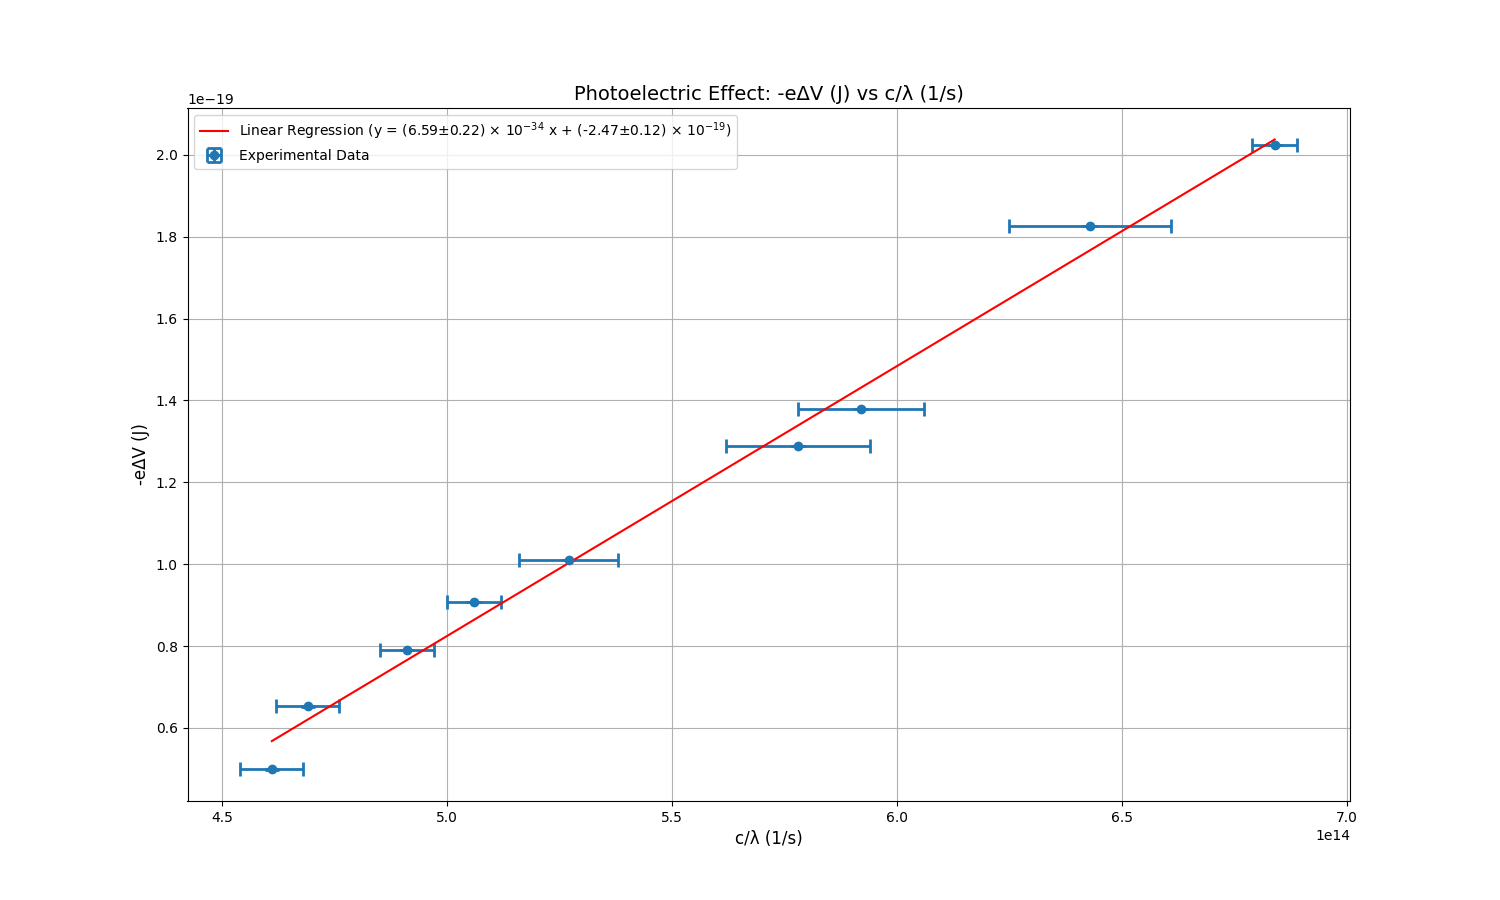
\includegraphics[width=0.8\textwidth]{../photoelectric_effect_plot.png}
  \caption{A plot of our measured values of $-e\Delta V$
    versus $\frac{c}{\lambda}$, with a linear trend line fitted to the
    data and the slope of the trend line providing an experimental
    value for Planck's constant: $h = (6.59 \pm 0.22) \times
    10^{-34}$ J·s. The intercept of the trend line provides an
    experimental value for the work function of the metal: $W = (2.47
  \pm 0.12) \times 10 ^{-19}$ J. Note: this figure does not include the origin.}
  \label{fig:photoelectric_plot}
\end{figure}

\begin{figure}[H]
  \centering
  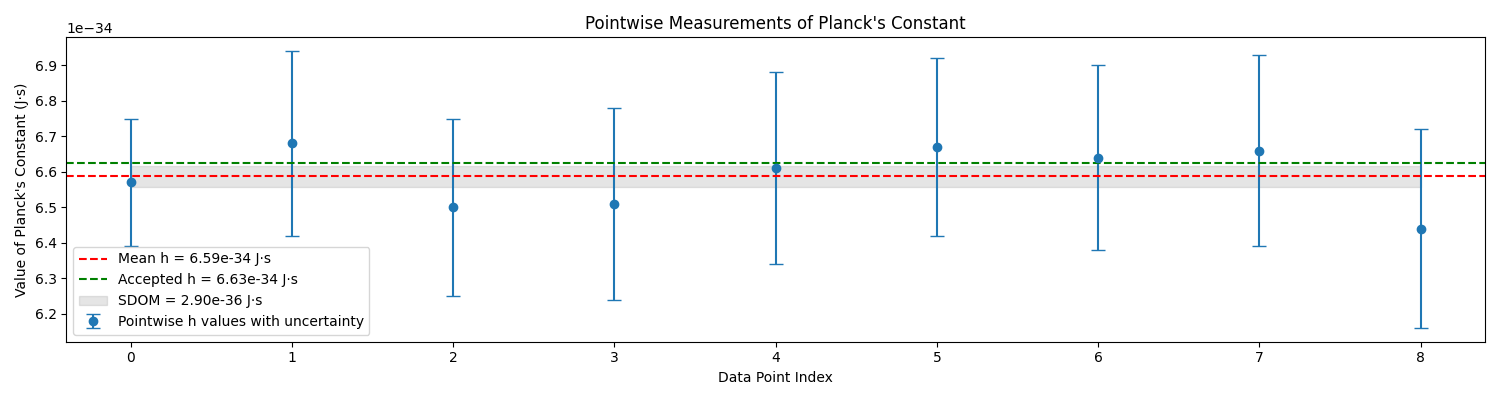
\includegraphics[width=0.8\textwidth]{../pointwise_h_values.png}
  \caption{A plot of our measured values of Planck's constant with measurement
    uncertainties, derived from single data points. The plot
    indicates the mean value across all measurements and the accepted value of
    Planck's constant. The mean provides our experimental value.
  }
  \label{fig:pointwise_h_values}
\end{figure}

The value for $h$ obtained from our regression analysis is $h +
\sigma _{h} =(6.59 \pm
0.22) \times 10^{-34}$
J·s, which is consistent with the accepted value of $6.626 \times 10^{-34}$
J·s to within $1 \sigma$. The value obtained from our pointwise analysis is
$\bar h + \sigma _{\bar h} = (6.587 \pm 0.029) \times 10^{-34}$ J·s, which is
consistent with the accepted value to approximately 1.35$\sigma$. Our
value for the work function of the photocell metal
$W$, $(2.47 \pm 0.12) \times 10^{-19}$ J = $(1.54 \pm 0.07)$ eV, is a
measure of the
effective work function
of the metal. This value is "effective" in the sense that the metal surface
contains impurities, which alters the states of the electrons on the
surface. The work function related to the photoelectric effect
is defined under the assumption that the metal surface is free from
such impurities [1].

We also note that the work function of our photocell metal does not
vary with light intensity,
in line with the quantum mechanical model of the photoelectric effect. Despite varying 
peak intensities of each light source used, assumptions that the work function

\vspace{1em}

We note that the centers of the values we find from linear regression and from
SDOM analysis are consistent with each other, but that the uncertainty of the
SDOM analysis is an order of magnitude smaller. We note that SDOM
analysis methods
often produce uncertainties that might be smaller than what one is
comfortable with
reporting, and accept the margin of agreement of $1.35\sigma$ as an appropriate
indicatior that our findings are consistent with the accepted value.

Our disagreement with the accepted value for Planck's constant might
be accounted for by
several sources of uncertainty: we note that there is a considerable amount
of electrical noise in the measurements of the picoammeter, that the initial
photocurrent was not stable at its initial value between all
wavelengths, and that
light sources often had intensity vs. wavelength relationships with significant
deviation from a Gaussian distribution. We identify the need to pursue a more
controlled method for setting and measuring photocurrents as well as
more appropriate models
for spectrogram measurements.

% TODO: cite

\section{Conclusion}

We obtain the values $h = (6.59 \pm 0.22) \times 10^{-34}$ and $h =
(6.587 \pm 0.029) \times 10^{-34}$ for Planck's constant, a fundamental quantity
describing the relationship between a photon's frequency and its
energy. We successfully
apply a procedure involving inducing the photoelectric interaction
between lights of several
wavelengths and a metal photocell, obtaining values in agreement with
the accepted CODATA value. Tangentially, we also determine an
effective work function
of our photocell metal: $(1.54 \pm 0.07)$ eV. Our work also includes
an investigation
of the relationship between the anode-cathode retarding voltage and
the post-gap photoelectric current produced.

\section{References}

[1] Harris, R. (2008). Modern Physics. Addison-Wesley.

\vspace{1em}

[2] Knight, Randall D, et al. College Physics. Addison-Wesley, 4 Jan. 2016.

\end{document}
